% ============================================================
% DIAGRAM: LSTM Cell (1997)
% ============================================================
% Caption: Figure 4.3: LSTM cell with CEC and gates.
%          (Adapted from Hochreiter & Schmidhuber, 1997, p. 1736)
% ============================================================

\documentclass[tikz,border=10pt]{standalone}
\usepackage{tikz}
\usepackage{amsmath}
\usepackage{amsfonts}

\usetikzlibrary{shapes,arrows,positioning,fit,calc,backgrounds}

\begin{document}

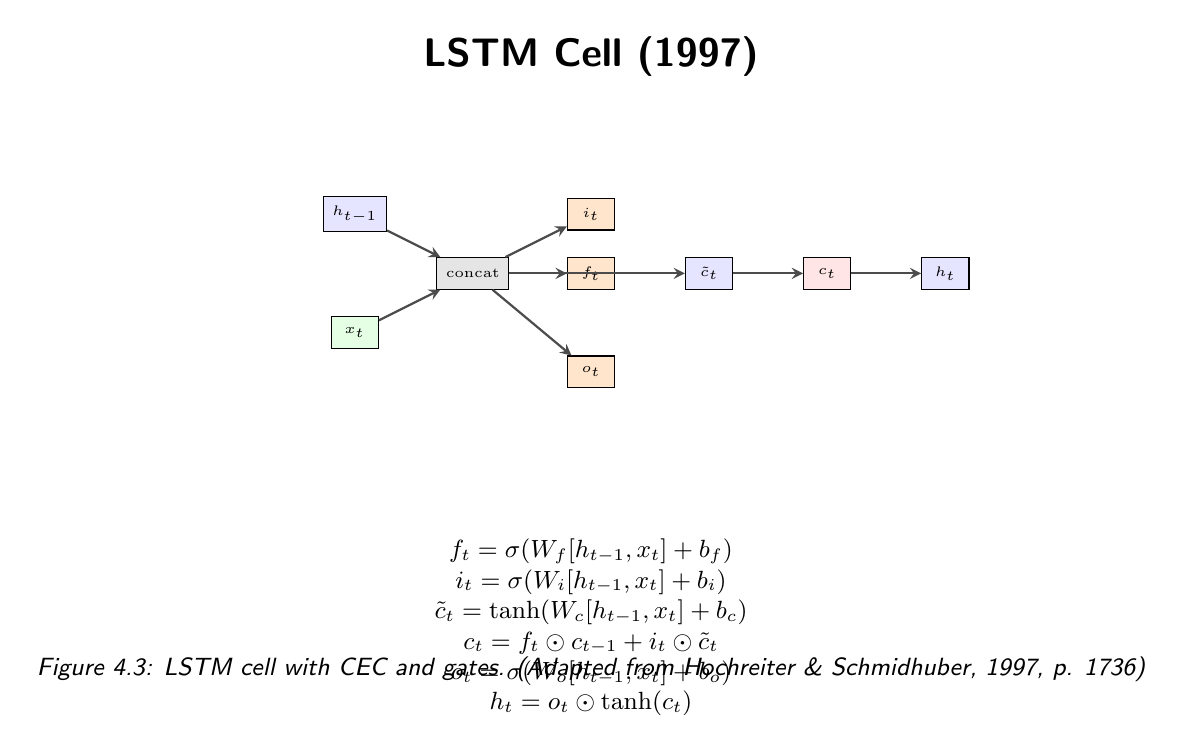
\begin{tikzpicture}[
    block/.style={draw, rectangle, minimum width=0.6cm, minimum height=0.4cm, fill=gray!20, font=\tiny},
    gate/.style={draw, rectangle, minimum width=0.6cm, minimum height=0.4cm, fill=orange!20, font=\tiny},
    neuron/.style={draw, circle, minimum size=0.4cm, inner sep=0pt, fill=blue!10},
    edge/.style={-stealth, thick, draw=black!70},
    label/.style={font=\sffamily\small},
    title/.style={font=\sffamily\Large\bfseries},
    caption/.style={font=\sffamily\small\itshape},
]

\node[title] at (0, 3.5) {LSTM Cell (1997)};

% Input
\node[block, fill=green!10] (x) at (-3, 0) {$x_t$};

% Previous hidden
\node[block, fill=blue!10] (hprev) at (-3, 1.5) {$h_{t-1}$};

% Combined input
\node[block, fill=gray!20] (combine) at (-1.5, 0.75) {concat};

% Gates
\node[gate] (input_gate) at (0, 1.5) {$i_t$};
\node[gate] (forget_gate) at (0, 0.75) {$f_t$};  % Note: forget gate added later, but we include for modern reference
\node[gate] (output_gate) at (0, -0.5) {$o_t$};

% Candidate cell
\node[block, fill=blue!10] (candidate) at (1.5, 0.75) {$\tilde{c}_t$};

% Cell state
\node[block, fill=red!10] (cell) at (3, 0.75) {$c_t$};

% Hidden output
\node[block, fill=blue!10] (hout) at (4.5, 0.75) {$h_t$};

% Edges (simplified)
\draw[edge] (x) -- (combine);
\draw[edge] (hprev) -- (combine);
\draw[edge] (combine) -- (input_gate);
\draw[edge] (combine) -- (forget_gate);
\draw[edge] (combine) -- (candidate);
\draw[edge] (combine) -- (output_gate);
\draw[edge] (candidate) -- (cell);
\draw[edge] (cell) -- (hout);

% Equations
\node[align=center, font=\sffamily\small, anchor=north] at (0, -2.5) {
  $f_t = \sigma(W_f [h_{t-1}, x_t] + b_f)$ \\
  $i_t = \sigma(W_i [h_{t-1}, x_t] + b_i)$ \\
  $\tilde{c}_t = \tanh(W_c [h_{t-1}, x_t] + b_c)$ \\
  $c_t = f_t \odot c_{t-1} + i_t \odot \tilde{c}_t$ \\
  $o_t = \sigma(W_o [h_{t-1}, x_t] + b_o)$ \\
  $h_t = o_t \odot \tanh(c_t)$
};

\node[caption, anchor=north] at (0, -4.0) {
  Figure 4.3: LSTM cell with CEC and gates. (Adapted from Hochreiter \& Schmidhuber, 1997, p. 1736)
};

\end{tikzpicture}
\end{document}
